\documentclass[hyperref={dvipdfmx,pdfpagelabels=false}]{beamer}
\title{Einführung in Matlab - Einheit 5}
\subtitle{Mehrdimensionale Arrays, Funktionen, Dünnbesetzte Matrizen, Numerische Mathematik}
\mode<article>
{
  \usepackage{fullpage}
  \usepackage{pgf}
  \usepackage{hyperref}
  \setjobnamebeamerversion{beamer}
}

\mode<presentation>
{
  %\usetheme{Frankfurt}
 %\usetheme{My}
  \usetheme{Madrid}
  % or ...
%\usecolortheme{seagull}
  %\setbeamercovered{transparent}
  %\setbeamercovered{dynamic}
  % or whatever (possibly just delete it)
}
\usenavigationsymbolstemplate{}
\usefonttheme{structurebold}
\usepackage{multimedia}
\usepackage{tikz}
\usepackage{fontspec,xunicode,xltxtra}
%\usepackage[scaled=.90]{helvet}
% Or whatever. Note that the encoding and the font should match. If T1
% does not look nice, try deleting the line with the fontenc.

\setbeamertemplate{footline}
{
\leavevmode
%\hbox{\begin{beamercolorbox}[wd=.5\paperwidth,ht=2.5ex,dp=1.125ex,
%leftskip=.3cm plus1fill,rightskip=.3cm]{author in head/foot}%
%    \usebeamerfont{author in head/foot}\insertshortauthor
%  \end{beamercolorbox}%
%  \begin{beamercolorbox}[wd=.5\paperwidth,ht=2.5ex,dp=1.125ex,leftskip=.3cm,
%rightskip=.3cm plus1fil]{title in head/foot}%
%    \usebeamerfont{title in head/foot}\insertshorttitle\hfill

\hfill\insertframenumber  \hspace{3pt}

%\inserttotalframenumber
%\hspace*{2ex}
%  \end{beamercolorbox}}%
  \vskip3pt%
}

%\usepackage[english]{babel}
\usepackage[ngerman]{babel}
\selectlanguage{ngerman}

%
% math/symbols
%
\usepackage{amssymb}
\usepackage{amsthm}
% \usepackage{latexsym}
\usepackage{amsmath}
%\usepackage{listings}
\usepackage[framed]{mcode}
%\usepackage{mcode}

\usepackage{mydef}
\usepackage{cmap} % you can search in the pdf for umlauts and ligatures
%\usepackage{colonequals} %corrects the definition-symbols \colonequals (besides others)
\title{Einführung in Matlab}
%
%\subtitle{Disputation} % (optional)

\author{Jochen Schulz}
% - Use the \inst{?} command only if the authors have different
%   affiliation.

\institute{Georg-August Universit\"at G\"ottingen \pgfimage[height=0.5cm]{../figures/unilogo3}}
% - Use the \inst command only if there are several affiliations.
% - Keep it simple, no one is interested in your street address.

\date{\today}

\subject{Einführung in Matlab}
% This is only inserted into the PDF information catalog. Can be left
% out. 



% If you have a file called "university-logo-filename.xxx", where xxx
% is a graphic format that can be processed by latex or pdflatex,
% resp., then you can add a logo as follows:

%\logo{\pgfimage[height=0.5cm]{figures/unilogo3}}


% Delete this, if you do not want the table of contents to pop up at
% the beginning of each subsection:
% \AtBeginSubsection[]
% {
%   \begin{frame}<beamer>
%     \frametitle{Aufbau}
%     \tableofcontents[currentsection,currentsubsection]
%   \end{frame}
% }

\AtBeginSection[]
{
  \begin{frame}<beamer>
    \frametitle{Aufbau}
    \tableofcontents[currentsection,currentsubsection]
  \end{frame}
}


\begin{document}



\maketitle

\section{Mehrdimensionale Arrays}
%
%
% Slide: 
%
\begin{frame}[fragile]\frametitle{Mehrdimensionale Arrays}
\begin{itemize}
\item mehrdimensionale Arrays (Dim. > 2).
\begin{lstlisting}
A(:,:,1) = ones(3);
A(:,:,2) = 2*ones(3);
whos
\end{lstlisting}
\begin{matlab}
  Name   Size   Bytes  Class  
  A      3x3x2    144  double  
\end{matlab}
\item \alert{ \mcode{cat(<dim>,<A1>,<A2>,..)}} f\"ugt die Arrays \mcode{A1},
  \mcode{A2},.. entlang der Dimension \mcode{dim} zusammen. 
\begin{lstlisting}
 A = cat(3,ones(3), 2*ones(3))
\end{lstlisting}
\item Befehle wie \alert{ \mcode{zeros}}, \alert{ \mcode{ones}} oder \alert{
  \mcode{repmat}} funktionieren auch im multidimensionalen Kontext.
\end{itemize}
\end{frame}
%
% Slide: 
%
\begin{frame}[fragile]\frametitle{Umsortieren von Arrays}
\begin{lstlisting}
reshape(X,n1,..,ns)
\end{lstlisting}
Der Befehl liest $X$ spaltenweise
aus, und schreibt die Elemente spaltenweise in ein $(n_1, \dots,
n_s)$-Array. 
\begin{itemize}
\item $X$ muss $n_1 \cdots n_s$ Elemente enthalten.
\item Der Befehl ist sehr n\"utzlich.
\end{itemize}
\textbf{Beispiele:}
\begin{lstlisting}
reshape(hilb(4), 8,2)
reshape(hilb(4), 4,2,2)
\end{lstlisting}
\end{frame}
%
% Slide: 
%
\begin{frame}[fragile]\frametitle{Zugriff auf mehrdim. Arrays}
Intern werden Arrays als Spalten abgespeichert. Zugriff durch linearen
  Index m\"oglich. 
\begin{lstlisting}
B = reshape(1:12,2,3,2)
\end{lstlisting}
\begin{matlab}
B(:,:,1) =
     1     3     5
     2     4     6
B(:,:,2) =

     7     9    11
     8    10    12
\end{matlab}
\begin{lstlisting}
B(7:9)
\end{lstlisting}
\begin{matlab}
ans =
     7     8     9
\end{matlab}
\end{frame}
%
% Slide
% 
\begin{frame}[fragile]\frametitle{N\"utzliche Befehle}
\begin{itemize}
\item Anzahl der Dimensionen von $X$: 
\begin{lstlisting}
ndims(X) 
\end{lstlisting}
\item Gr\"o{\ss}e von $X$: 
\begin{lstlisting}
size(X)
\end{lstlisting}
\item Umwandlung von linearer Indizierung in Array-Indizierung: 
\begin{lstlisting}
ind2sub
\end{lstlisting}
\item Umwandlung von Array-Indizierung in lineare Indizierung:
 \begin{lstlisting}
sub2ind
\end{lstlisting}
\begin{lstlisting}
A = reshape(1:12,2,3,2);
A(ind2sub(size(A),5))
\end{lstlisting}
\begin{matlab}
ans =
     5
\end{matlab}
\item Man kann auch mit mehrdimensionalen Arrays rechnen.
\end{itemize}

\end{frame}
%



\section{Funktionen}

%
% Slide
%
\begin{frame}[fragile]\frametitle{Funktionen}
\begin{itemize}
 \item Funktions-Typen
\begin{itemize}
\item m.-File
\item inline
\item anonyme
\item string
\end{itemize}
\item Funktionen werden in einem eigenen {\it Workspace} verwaltet.
\item Beim ersten Aufruf speichert MATLAB die Funktion im Workspace bis MATLAB
  verlassen wird oder die Funktion \mcode{fun} mit  \mcode{clear fun} gel\"oscht wird.
\item Namen: Buchstaben mit 1-63 Zeichen (Ohne -,+,*,/ !). 
\end{itemize}
\end{frame}

%
% Slide
%
\begin{frame}[fragile]\frametitle{Function-Handles}

Ein {\it Function Handle} ist ein MATLAB Datentyp, das alle Informationen
enth\"alt, die zur Auswertung einer Funktion n\"otig sind.\\
\begin{itemize}
\item Definition, z.B. 
\begin{lstlisting}
Sinus = @sin 
\end{lstlisting}
\item Anwendung bei der \"Ubergabe von Funktionen:
\begin{lstlisting}
quad(Sinus,0,1)
\end{lstlisting}
\item m-File Funktionen haben ihren Namen als Handle ( \mcode{@func_name} für \mcode{func_name.m})
% \item Anonyme Funktion: 
% \begin{lstlisting}
%  f = @(x) sin(x)*cos(x)
% \end{lstlisting}
\end{itemize}
\end{frame}


\subsection{Ein-/Ausgabe - Parameter}
%
% Slide
%
\begin{frame}[fragile]\frametitle{Ein-/Ausgabe - Parameter} 
\begin{itemize}
 \item Eingabeparameter als Cell-Array
\begin{lstlisting}
varargin
\end{lstlisting}
\item Die Anzahl der Inputvariablen
\begin{lstlisting}
nargin
\end{lstlisting}
\item Cell-Array der Ausgabewerte
\begin{lstlisting}
varargout
\end{lstlisting}
\item Die Anzahl der Outputvariablen
\begin{lstlisting}
nargout
\end{lstlisting}
\end{itemize}

\end{frame}
%
% Slide
%
\begin{frame}[fragile]\frametitle{Beispiel: varargin}
\begin{lstlisting}
function result = integral(varargin)
% berechnet approximativ ein Integral ueber (a,b) 
% durch die Mittelpunktregel mit Hilfe von N Punkten
% Eingabe: 0 Parameter:       (N=20, a=0, b=1)
%          1 Parameter: N     (a=0,b=1)
%          3 Parameter: N,a,b
% Jochen Schulz		16.08.2009
N = 20; a = 0; b = 1; % Default-Einstellung
anzahl_parameter = nargin; % Anz. Input-argumente
if anzahl_parameter == 1 
    N = varargin{1};
end
if anzahl_parameter == 3
    N = varargin{1}; a = varargin{2}; 
    b = varargin{3};
end
if anzahl_parameter ~= [0 1 3]
    error('Falsche Anzahl an Input-Argumenten');
end
\end{lstlisting}
\end{frame}
\begin{frame}[fragile]\frametitle{Beispiel: varargin}
\begin{lstlisting}
x = (a+(b-a)/(2*N)):(b-a)/N:(b-(b-a)/(2*N));
y = x.^3;
% Berechnung des Integrals
result = (b-a)*sum(y)*(1/N);

close all; % Plot
x1 = linspace(a,b,N+1);
for i = 1:N
    fill([x1(i) x1(i)  x1(i+1) x1(i+1)], [0 y(i)  y(i) 0], 'r');
    hold on;
end
plot(a:(b-a)/100:b,(a:(b-a)/100:b).^3,'LineWidth',3);
title(strcat('\int x^3 = ',num2str(result),...
' fuer N =', num2str(N))); 
\end{lstlisting}
\end{frame}


\subsection{Funktionen-Typen}
%
% Slide
%
\begin{frame}[fragile]\frametitle{Anonyme Funktion}
\begin{lstlisting}
 @(<x>) <funktion(x)>
\end{lstlisting}

\begin{itemize}
\item Funktion mit Parameter
\begin{lstlisting}
y = 1; f = @(x) sin(x)./(x+y) ;
f(2)
\end{lstlisting}
\begin{matlab}
ans =
    0.3031
\end{matlab}

\item Gamma-Funktion $\Gamma(s) = \int_0^\infty x^{s-1} e^{-x} dx$.
\begin{lstlisting}
k = @(s) quad( @(x) x.^(s-1).*exp(-x),0.1,500) ;
k(4),k(5)
\end{lstlisting}
\begin{matlab}
ans =
    6.0000
ans =
   24.0000
\end{matlab}

\end{itemize}
\end{frame}

%
% Slide
%
\begin{frame}[fragile]\frametitle{String-Funktionen}
\begin{lstlisting}
<fun> = '<funktions-string>' 
\end{lstlisting}

\begin{itemize}
\item Eingabe als String: 
\begin{lstlisting}
a = 'exp(z)-1+z'
\end{lstlisting}
\item Plotten der zugeh\"origen Funktion 
\begin{lstlisting}
ezplot(a,[-1 1]) 
\end{lstlisting}
%\item Konvertieren zwischen Strings und Funktionen: \alert{
%  \mcode{str2func}}, \alert{ \mcode{func2str}} 
\end{itemize}
\alert{Bemerkung:} \\
Funktionen gegeben als Strings sind im allgemeinen zu vermeiden!
Besser andere Konstrukte (wie Inline-Funktionen) benutzen!
\end{frame}



%
% Slide
%
\begin{frame}[fragile]\frametitle{Inline-Funktionen}
\begin{lstlisting}
<fun> =  inline('<funktions-string>')
\end{lstlisting}

\textbf{Beispiele:} \\
\begin{columns}[t]
 \column{0.48\textwidth}
\begin{lstlisting}
a = 'exp(z) - 1 + z'; 
f = inline(a)
\end{lstlisting}
\begin{matlab}
f =
     Inline function:
     f(z) = exp(z)-1+z
\end{matlab}
\begin{lstlisting}
g = inline('x+y^2','x','y')
\end{lstlisting}
\begin{matlab}
g =
     Inline function:
     g(x,y) = x+y^2
\end{matlab}
\column{0.48\textwidth}
\begin{lstlisting}
f(1),g(1,2),a(2)
\end{lstlisting}
\begin{matlab}
ans =
    2.7183
ans =
     5
ans =
     x
\end{matlab}
\end{columns}
\end{frame}

\subsection{Umgang und Beispiele}
%
% Slide
%
\begin{frame}[fragile]\frametitle{Befehle f\"ur Funktionen}
\begin{itemize}
\item Auswertung der Funktion  \mcode{fun} an der Stelle $(x1,..,xn)$. 
\begin{lstlisting}
feval(<fun>,<x1>,..,<xn>)
\end{lstlisting}
\mcode{fun} ist dabei
  entweder ein Funktionsname oder ein Function-Handle. 
\item Wandlung eines Strings \mcode{g} in eine Inline-Funktion (vgl. \mcode{inline}). 
\begin{lstlisting}
f = fcnchk(<g>) 
\end{lstlisting}
Ist \mcode{g} ein
  Function-Handle oder eine Inline-Funktion so ist $f = g$.  

\item Strings oder Inline-Funktionen \mcode{f} \textsl{vektorisieren}
\begin{lstlisting}
vectorize(<f>)
\end{lstlisting}
d.h. \mcode{'*'} $\Rightarrow$ \mcode{'.*'} , \mcode{'^'} $\Rightarrow$ \mcode{'.^'}, usw. 

\end{itemize}
\end{frame}
%
% Slide
%
\begin{frame}[fragile]\frametitle{Beispiel: integral2.m (Auszug)}
\begin{lstlisting}
function result = integral2(varargin)
% Eingabe: 1 Parameter: f       (N=20, a=0, b=1)
%          2 Parameter: f,N     (a=0,b=1)
%          4 Parameter: f,N,a,b
N = 20; a = 0; b = 1; % Default-Einstellung
anzahl_parameter = nargin; % Anz. Input-argumente
if anzahl_parameter == 2 
    N = varargin{2};
end;
if anzahl_parameter == 4
    N = varargin{2}; a = varargin{3}; b = varargin{4};
end;
if anzahl_parameter ~= [1 2 4]
    error('Falsche Anzahl an Input-Argumenten');
end;
% eventuelle Umwandlung von Strings
f = fcnchk(varargin{1},'vectorized'); 
x = (a+(b-a)/(2*N)):(b-a)/N:(b-(b-a)/(2*N));
y = feval(f,x);  
\end{lstlisting}
\end{frame}
% 
% Slide
% 
\begin{frame}[fragile]\frametitle{}
\centering\alert{ \mcode{integral2('log(x.^2)',30,1,5)}}\\
\begin{center}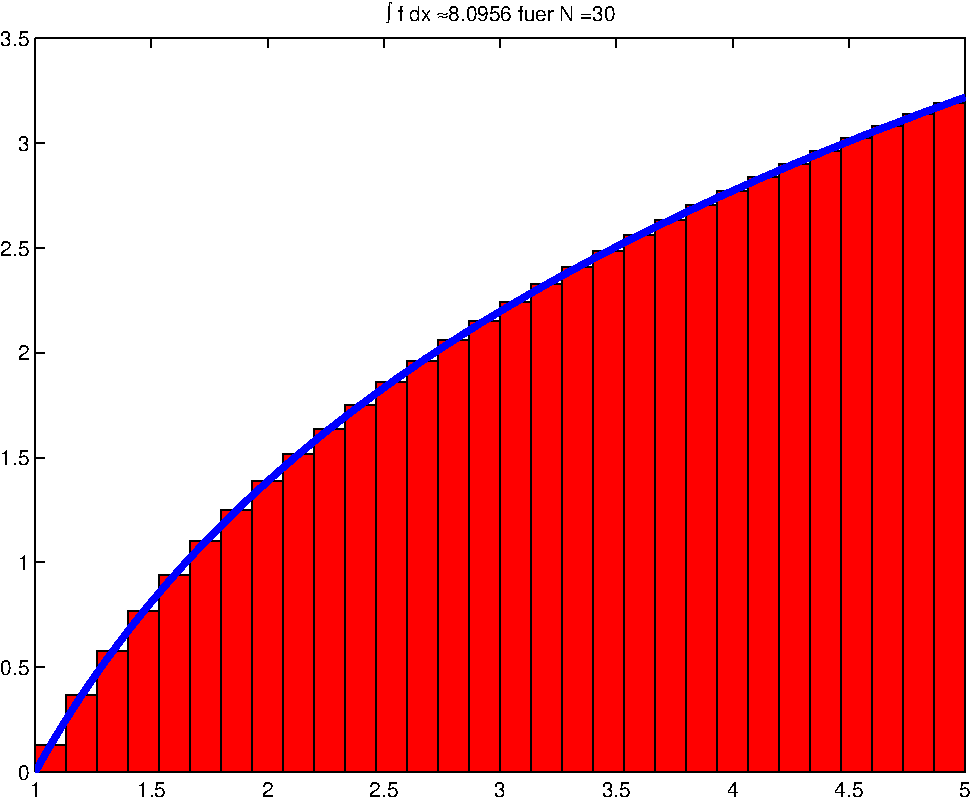
\includegraphics[width=0.8\textwidth]{./figures/plot_log}\end{center} 
\end{frame}



%
% Slide
%
\begin{frame}[fragile]\frametitle{Beispiel: Sobolevsche Mittelungsfunktion}
\alert{ \[ f(x) := \left \{ \begin{array}{ll} \exp(- \frac{1}{1-\|x\|^2}), &
\|x \| <1 \\ 0, & \|x \| \geq 1 
\end{array} \right .  
\]}
mit $\|x\|^2:=\sum_{i=1}^N x_i^2$, $x=(x_1, \dots x_N) \in
\mathbb{R}^N$.\\[0.5cm]

2 Versionen:
\begin{itemize}
\item eindimensionale Version
\item N-dimensionale Version
\end{itemize}
\end{frame}
%
% Slide
%
\begin{frame}[fragile]\frametitle{1d-Fall}
\lstinputlisting{f_1d.m}
\end{frame}
%
% Slide
%
\begin{frame}[fragile]\frametitle{n-dimensionaler-Fall}
\begin{lstlisting}
function result = f(varargin)
% f.m     Sobolevsche Mittelungsfunktion
%         Eingabe: Matrizen x1,x2,x3,..
%         Ausgabe: Matrix result=f(x1,x2,...)
betrag = varargin{1}.^2;
for i = 2:nargin
  betrag = betrag+varargin{i}.^2;
end
dimension = size(varargin{1});
result = zeros(dimension(1),dimension(2));
for j = 1:dimension(1)
  for k = 1:dimension(2)
    if betrag(j,k) < 1
      result(j,k) = exp(-1/(1-betrag(j,k)));
    else
      result(j,k) = 0;
    end;
  end;
end;
\end{lstlisting}
\end{frame}
%
% Slide
%
\begin{frame}[fragile]\frametitle{Programm zum Plotten}
\begin{lstlisting}
%    plot_f.m

% Eindimensionaler Plot
subplot(2,2,1),
ezplot(@f);

% Zweidimensionaler Plot
subplot(2,2,2),
ezmesh(@f);

% Zweidimensionaler Plot
subplot(2,2,3),
ezsurfc(@f);

% Zweidimensionaler Plot
subplot(2,2,4),
ezcontourf(@f);
\end{lstlisting}
\end{frame}
\begin{frame}[fragile]\frametitle{Plots der Funktion}
\begin{center}
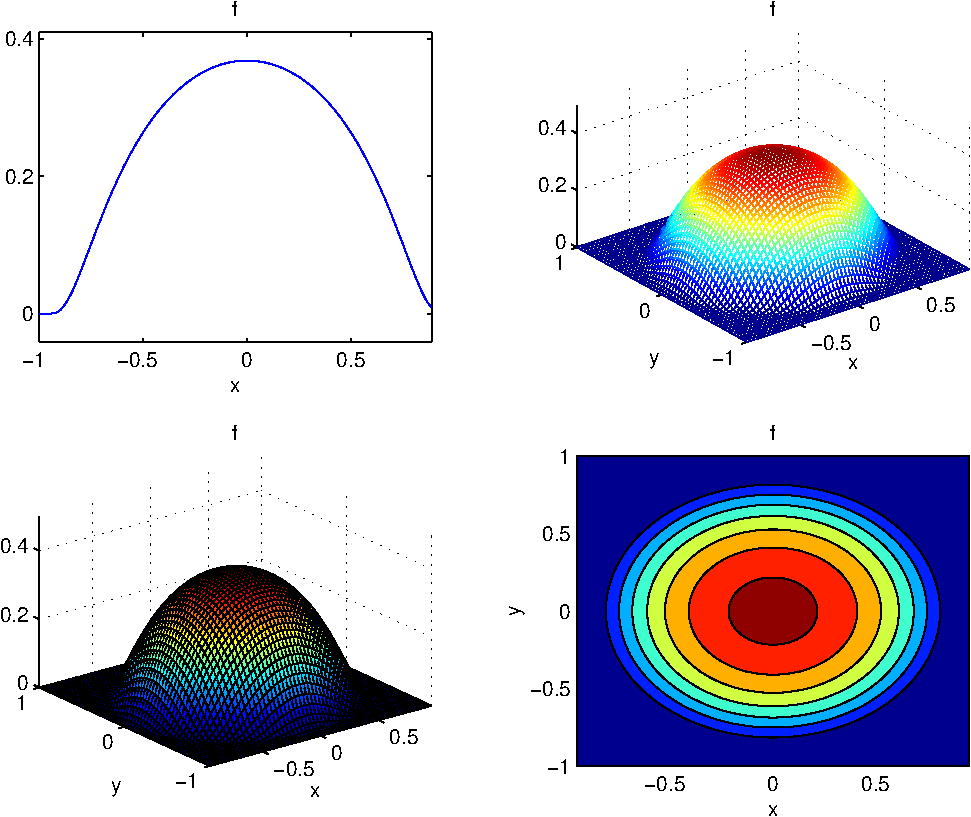
\includegraphics[width=0.8\textwidth]{./figures/plot_f}  
\end{center}
\end{frame}

% 
% Slide
% 
\begin{frame}[fragile]\frametitle{}
\centering\alert{ \mcode{integral2(@f,50,-1.1,1.1)}}\\
\begin{center}
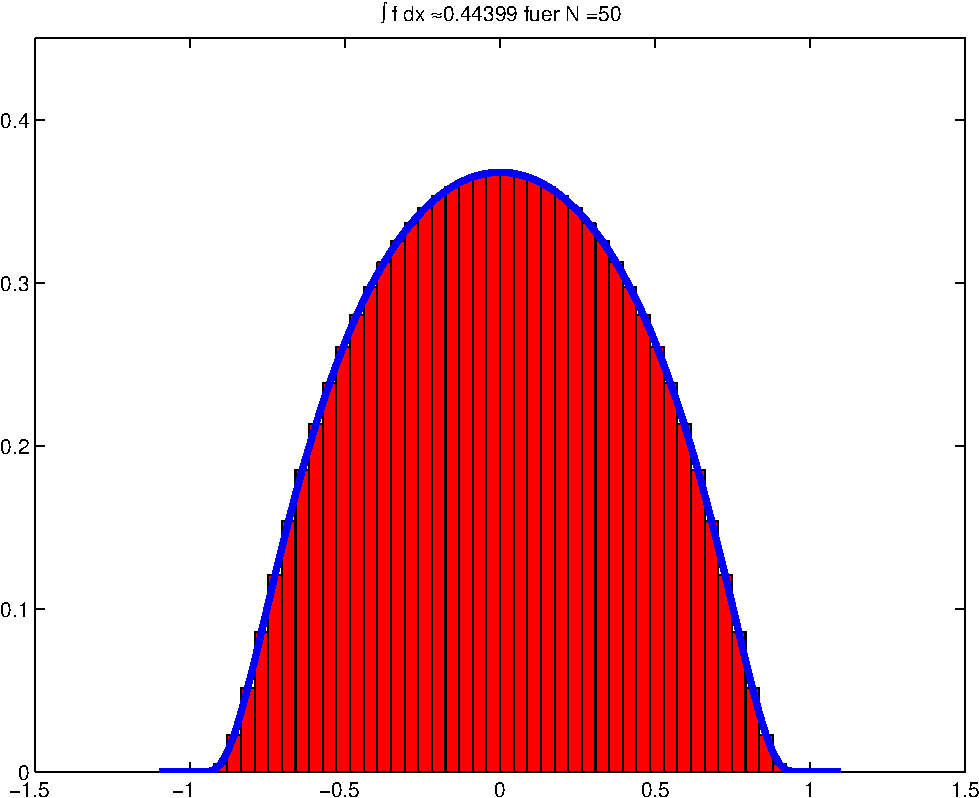
\includegraphics[width=0.8\textwidth]{./figures/plot_sobolev} 
\end{center}
\end{frame}

\section{D\"unnbesetzte Matrizen}

% 
% Slide 
%
\begin{frame}[fragile]\frametitle{D\"unnbesetzte Matrizen}
\begin{itemize}
\item Bei {\it D\"unnbesetzten Matrizen} ({\it sparse matrices}) sind
  fast alle Eintr\"age $0$.
\item In vielen Anwendungen, z.B. bei der Diskretisierung von
  Differentialgleichungen oder in der Graphentheorie, treten sehr
  grosse, d\"unnbesetzte  Matrizen auf.
\item In MATLAB steht daf\"ur ein eigener Datentyp zur Verf\"ugung, der zu
  jedem Nichtnullelement der Matrix, die zugeh\"orige Zeile und Spalte
  speichert.    
\end{itemize}
\end{frame}
% 
% Slide 
%
\begin{frame}[fragile]\frametitle{Beispiel}
\begin{lstlisting}
A = 2*diag(ones(10,1),0) ...
       - diag(ones(9,1),-1) ...
       - diag(ones(9,1),1);
B = sparse(A)
\end{lstlisting}
\begin{matlab}
B =   (1,1)        2
      (2,1)       -1
      (1,2)       -1
      (2,2)        2
\end{matlab}
\begin{lstlisting}
C = 2*diag(ones(100,1),0) ...
       - diag(ones(99,1),-1) ...
       - diag(ones(99,1),1);
D = sparse(C); whos
\end{lstlisting}
\begin{matlab}
  Name      Size           Bytes  Class
  A        10x10             800  double array
  B        10x10             380  sparse array
  C       100x100          80000  double array
  D       100x100           3980  sparse array
\end{matlab}
\end{frame}
% 
% Slide 
%
\begin{frame}[fragile]\frametitle{Einige Befehle}
\begin{itemize}
\item Erzeugung einer d\"unnbesetzten Matrix
  der Gr\"osse $n \times m$. Alle Eintr\"age sind $0$.
\begin{lstlisting}
sparse(n,m) 
\end{lstlisting}

\item Konvertierung der dichtbesetzten Matrix
  $A$ in eine d\"unnbesetzte Matrix.
\begin{lstlisting}
sparse(A)
\end{lstlisting}

\item Die Struktur der Matrix $A$ visualisieren.
\begin{lstlisting}
spy(A)
\end{lstlisting}

\item Die meisten Standardoperationen funktionieren auch mit
  d\"unnbesetzten Matrizen.  
\end{itemize}
\end{frame}
% 
% Slide 
%
\begin{frame}[fragile]\frametitle{Dichte und d\"unnbesetzte Matrizen}
\begin{itemize}
\item Konvertierung der d\"unnbesetzten Matrix $A$ in eine dichtbesetzte Matrix $B$ .
\begin{lstlisting}
B = full(A)
\end{lstlisting}
\item Bei bin\"aren Operationen, z.B. $A+B$ oder $A*B$ ist das Ergebnis
  bei d\"unnbesetzten Matrizen $A$ und $B$ wieder eine d\"unnbesetzte
  Matrix. \\Ist eine der Matrizen dichtbesetzt, so ist auch das Ergebnis
  dichtbesetzt. 
\item Berechnung der $k$ betragsm\"a{\ss}ig  gr\"ossten Eigenwerte (Default: $k=6$):
\begin{lstlisting}
eigs(A,k) 
\end{lstlisting}

\end{itemize}
\end{frame}
% 
% Slide 
%
\begin{frame}[fragile]\frametitle{D\"unnbesetzte Matrizen}
\begin{itemize}
\item Norm- und Konditionsberechnung:
\begin{lstlisting}
normest(<A>) , condest(<A>)
\end{lstlisting}

\item Alle iterativen Verfahren funktionieren auch mit d\"unnbesetzten
  Matrizen. 
\item Indizes aller Zeilen und Spalten erhalten, in denen Nichtnullelemente stehen: 
\begin{lstlisting}
[I,J] = find(X)
\end{lstlisting}
\item Eine \"Ubesicht aller Funktionen f\"ur d\"unnbesetzte Matrizen erh\"alt
  man durch \alert{ \mcode{help sparfun}}.  
\end{itemize}
\end{frame}

\section{Numerische Mathematik}

\subsection{Poisson Problem}
%
% Slide
% 
\begin{frame}[fragile]\frametitle{Poisson Problem}
\begin{itemize}
\item Poisson Problem beschreibt station\"are W\"armeverteilungen.
\item {\it Poisson Problem:} Suche  $u \in
C^2(\Omega)\cap C(\overline{\Omega})$ mit
\[
\left \{ \begin{array}{rcll}
- \triangle u & = & f & \mbox{in } \Omega\\
u & = & 0 & \mbox{auf } \partial \Omega\\ 
\end{array} \right.
\]
f\"ur $\Omega=(0,1)^2$ und $f \in C(\Omega)$.
\item  {\it Laplace-Operator} 
$ \triangle u := \sum_{i=1}^d \frac{\partial ^2 u}{\partial x_i^2} $
\end{itemize}
\end{frame}
%
% Slide
% 
\begin{frame}[fragile]\frametitle{Diskretisierung}
\begin{itemize}
\item \"Aquidistante Gitterweite $h= \frac 1 N$,
$N \in \mathbb{N}$
\item Menge aller Gitterpunkte 
\[ Z_h := \left\{ (x,y) \in \overline{\Omega} \ \mid \ x=z_1h, \ y=z_2h \text{ mit }
z_1,z_2 \in \mathbb{Z} \right\}. \]
\item Innere Gitterpunkte: $\omega_h := Z_h \cap \Omega$
\end{itemize}
\end{frame}
%
% Slide
% 
\begin{frame}[fragile]\frametitle{Diskretisierung}
\begin{itemize}
\item Approximation von $ \frac{\partial ^2 u}{\partial
  x^2} (x,y)$
{\small \[ \frac{u(x -h,y) - 2 u(x,y) + u(x+h,y)}{h^2} = \frac{\partial ^2 u}{\partial
  x^2} (x,y) + \mathcal{O}(h^2) \]}
\item  Approximation von $ \frac{\partial ^2 u}{\partial
  y^2} (x,y)$
{\small \[ \frac{u(x ,y-h) - 2 u(x,y) + u(x,y+h)}{h^2} = \frac{\partial ^2 u}{\partial
  y^2} (x,y) + \mathcal{O}(h^2) \]}
\item Addition ergibt f\"ur $ \triangle u(x,y)$ die N\"aherung
{\footnotesize \[
 \frac{1}{h^2} \left( u(x,y-h) + u(x-h,y) - 4 u(x,y) + u(x,y+h) +
 u(x+h,y)  \right) 
\] }
\end{itemize}
\end{frame}
%
% Slide
% 
\begin{frame}[fragile]\frametitle{Diskretisierung}
\begin{itemize}
\item Definition $u_{i,j}:=u(ih,jh)$ ergibt an Gitterpunkten $(ih,jh)$
\[ -u_{i,j-1} - u_{i-1,j} + 4 u_{i,j} - u_{i+1,j} - u_{i,j+1} = h^2 f_{ij} \] 
mit $i,j \in \{ 1, \dots , N-1 \}$ und $f_{ij}:=f(ih,jh)$. 
\item Randbedingungen ergeben
$u_{0,i}=u_{N,i}=u_{i,0}=u_{i,N}=0$, $i=0, \dots ,N$.
\end{itemize}
\end{frame}

%
% Slide
% 
\begin{frame}[fragile]\frametitle{Diskretisierung}
\begin{itemize}
\item Lexikografische Sortierung der inneren Unbekannten 
{\small \[ \begin{array}{cccc}
(h,(N-1)h) & (2h,(N-1)h) & \hdots & ((N-1)h,(N-1)h)\\
\vdots & \vdots & \vdots & \vdots \\
(h,2h) & (2h,2h) & \hdots & ((N-1)h,2h)\\
(h,h), & (2h,h) & \hdots & ((N-1)h,h)\\
\end{array} \]
}
ergibt Vektor $U_{i+(N-1)(j-1)}=u_{i,j}$.
\end{itemize}
\end{frame}
%
% Slide
% 
\begin{frame}[fragile]\frametitle{Diskretisierung}
Lineares Gleichungssystem f\"ur $U=(U_i)_{i=1}^{(N-1)^2}$
\[ A U = F \]
mit 
\begin{itemize}
\item $F:=(f_i)_{i=1}^{(N-1)^2}$ mit $f_{i+(N-1)(j-1)}=f(ih,jh)$, $i,j \in \{1,
\dots ,N-1 \}$,
\item  \begin{eqnarray*} 
A & := & \frac{1}{h^2} tridiag(-I_{N-1}, T, -I_{N-1}) \in \mathbb{R}^{(N-1)^2
 \times (N-1)^2},\\
 T & := & tridiag(-1,4,-1) \in \mathbb{R}^{(N-1)\times (N-1)}. 
\end{eqnarray*}
\end{itemize}
\end{frame}
%
% Slide
% 
\begin{frame}[fragile]\frametitle{Implementierung}
\begin{lstlisting}
function loes = poisson (f,n)
f = fcnchk(f);
A = gallery('poisson',n-1); 
% Erzeuge rechte Seite und Mesh
mesh = zeros(2,(n-1)^2);
F = zeros((n-1)^2,1);
for i = 1:(n-1)
    for j = 1:(n-1)
        F(i+(n-1)*(j-1)) = (1/n)^2*f(i/n,j/n);
        loes.mesh(:,i+(n-1)*(j-1)) = [i/n; j/n]; 
    end
end
% Loese das lineare System
loes.x = A \ F;
\end{lstlisting}
\end{frame}
%
% Slide
% 
\begin{frame}[fragile]\frametitle{Implementierung}
\begin{lstlisting}

% Ergaenze Randbedingungen
loes.x = [ loes.x; zeros(4*(n+1),1)];
loes.mesh = [loes.mesh, [zeros(1,n+1); 0:1/n:1]];
loes.mesh = [loes.mesh, [ones(1,n+1);  0:1/n:1]];
loes.mesh = [loes.mesh, [0:1/n:1; ones(1,n+1)]];
loes.mesh = [loes.mesh, [0:1/n:1; zeros(1,n+1)]];

% Plotten
plot3(loes.mesh(1,:),loes.mesh(2,:),loes.x,'*');
figure;
[X,Y] = meshgrid(0:1/n:1,0:1/n:1);
Fi = TriScatteredInterp(loes.mesh(1,:)', loes.mesh(2,:)',loes.x,'linear');
Z = Fi(X,Y);
surf(X,Y,Z);
\end{lstlisting}
\end{frame}

\subsection{Differentialgleichungen}
%
% Slide
%
\begin{frame}[fragile]\frametitle{Gew\"ohnliche Differentialgleichungen}
Sei $I \subset \mathbb{R}$ ein Intervall. Bei einer gewöhnlichen Dgl. sucht man eine Funktion $y:I \
\longrightarrow \mathbb{R}^n$, so dass
\alert{ \[ \frac{d}{dt}y(t)=f(t,y(t)), t\in I\quad y(t_0)=y_0, \]}
wobei $y_0 \in \mathbb{R}^n$ ein vorgegebener Anfangswert an $t_0\in I$
und $f:I \times \mathbb{R}^n \longrightarrow \mathbb{R}^n$ die
rechte Seite ist. Au{\ss}erdem sei $ \frac{d}{dt}y(t) :=(\frac{\partial
  y_1(t)}{\partial t}, \dots, \frac{\partial
  y_n(t)}{\partial t})^t$. \\
\alert{Beispiele:}\\
{\scriptsize
$\frac{d}{dt} y(t) = y(t), \ y(t_0)=y_0$, \quad L\"osung:
$y(t)=y_0 e^{t-t_0}$\\
$\frac{d}{dt} y(t) = e^y \sin(t)$, \quad L\"osung: $y(t)=-\log( \cos(x)+C)$, $C+\cos(x)>0$ }
\end{frame}
%
% Slide
%
\begin{frame}[fragile]\frametitle{Skalares Beispiel}
L\"ose f\"ur $0 \leq t \leq 3$ mit \alert{ ode45} die Dgl.
\alert{ \[ \frac{d}{dt} y(t) = -y(t)-5e^{-t}\sin5t, \quad y(0)=1. \]}
\begin{itemize}
\item Die rechte Seite als eigene Funktion:
\begin{lstlisting}
function z = rechte_seite1(t,y)
% rechte_seite1   ODE Beispiel
%         z=rechte_seite1(t,y)
z = -y-5*exp(-t)*sin(5*t);
\end{lstlisting}
\end{itemize}
\end{frame}
%
% Slide
%
\begin{frame}[fragile]\frametitle{Skalares Beispiel}
\begin{itemize}
\item Ausrechnen und Plotten
\begin{lstlisting}
tspan = [0,3]; aw = 1;
[t,y] = ode45(@rechte_seite1,tspan,aw);
plot(t,y,'*--','Linewidth',3)
xlabel('t'), ylabel('y(t)')
\end{lstlisting}
\end{itemize}
\begin{center}
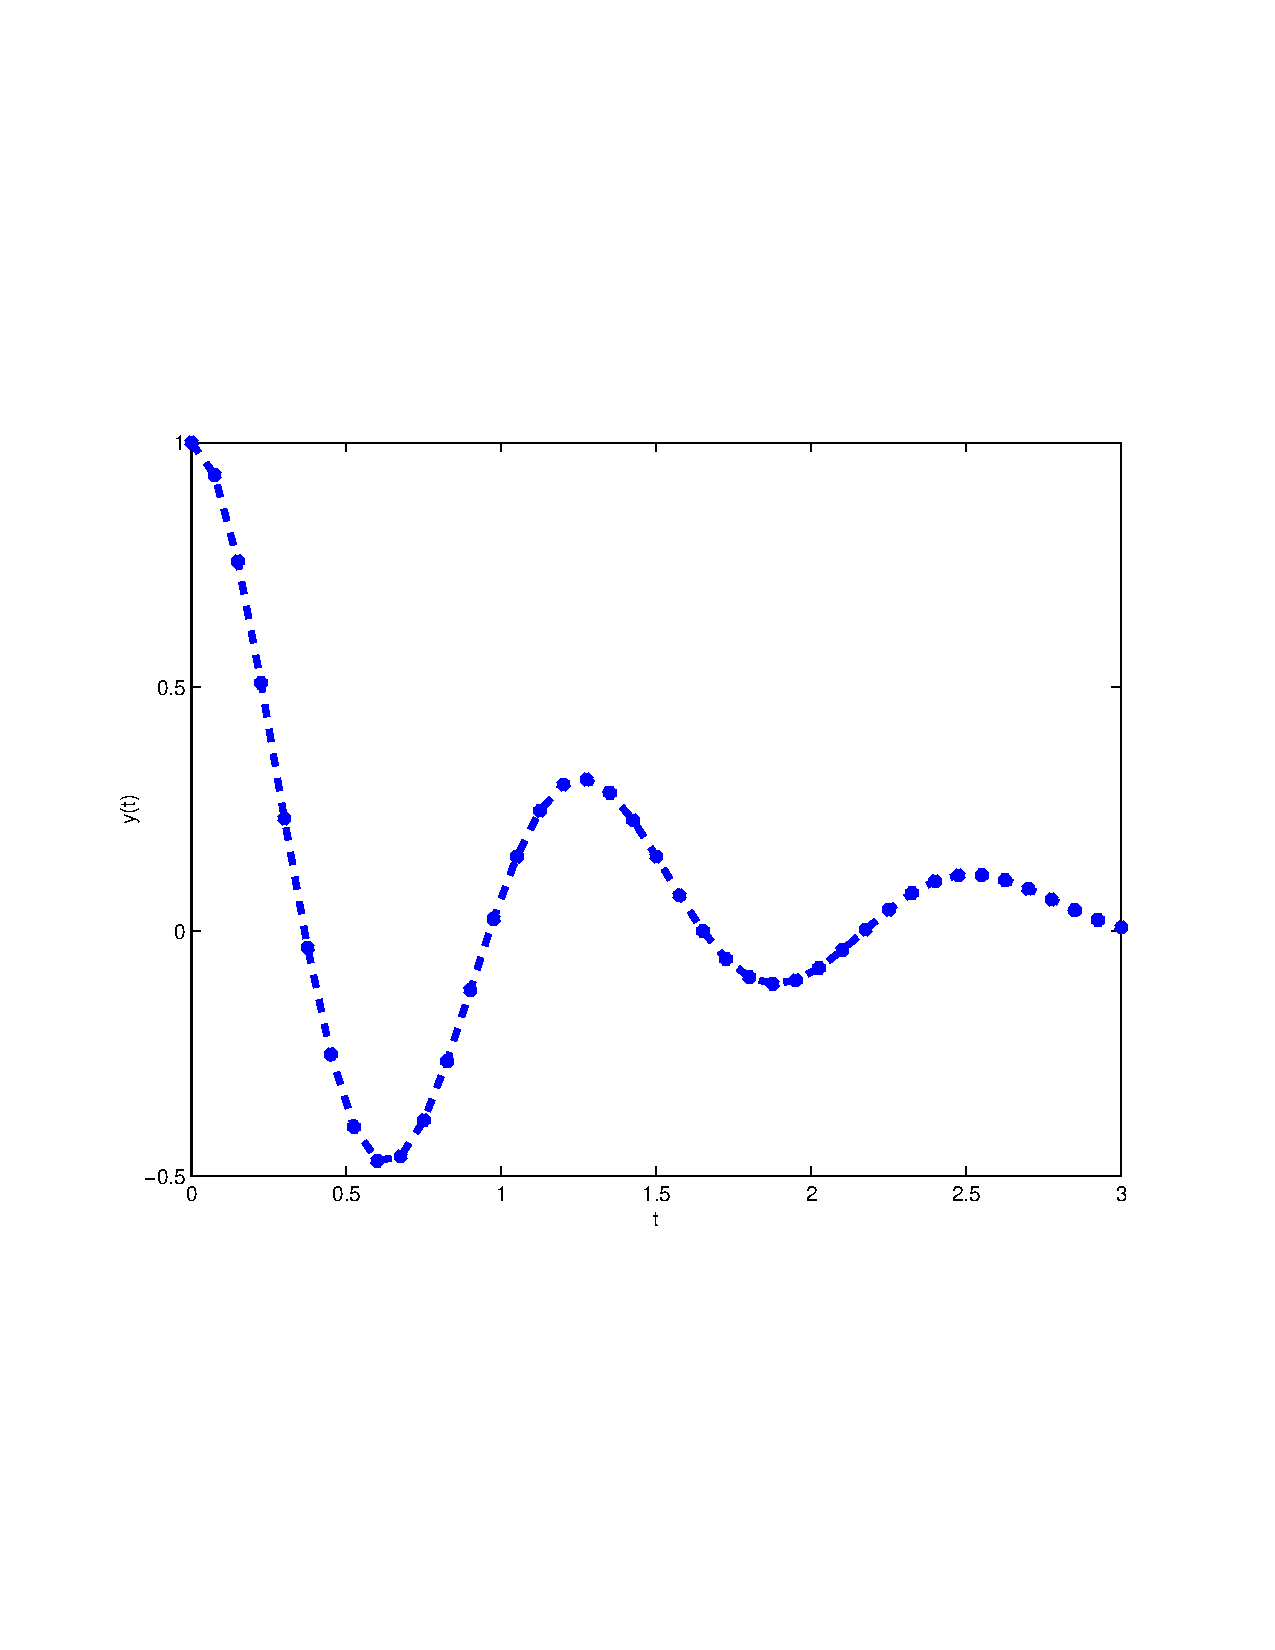
\includegraphics[width=0.5\textwidth]{./figures/loesung_dgl1} 
\end{center}
\end{frame}
%
% Slide
%
\begin{frame}[fragile]\frametitle{ODE in MATLAB} 
\begin{lstlisting}
[<t>,<y>] = ode45(<@fun>, <tspan>, <aw>, <options>)
\end{lstlisting}
\begin{itemize}
\item \mcode{@fun} steht f\"ur die rechte Seite der Dgl. (m-File).
\item $aw \in \mathbb{R}^n$ ist der Anfangswert.
\item $tspan$ gibt das Zeitintervall an, auf dem die Dgl. berechnet
  werden soll. Normalerweise ist es von der Form
  \mcode{tspan=[t_0, t_1]}. Dann wird die Dgl. auf dem Intervall $[t_0,
  t_1]$ berechnet (Anfangswert: $y(t_0)=aw$).
\item Rückgabewerte: Vektoren $t$ und Matrizen $y$. Dabei ist
  $y(:,i)$ die L\"osung an der Stelle $t(i)$. Die Punkte $t_i$ werden
  automatisch bestimmt.
\item Durch die optionale Angabe von \mcode{options} kann der L\"oser
  gezielt eingestellt werden. 
\item Spezifiziert man mehr als zwei Zeitpunkte in \mcode{tspan}, so gibt MATLAB die
  L\"osung genau an diesen Zeitschritten zur\"uck.
\end{itemize}
\end{frame}
%
% Slide
%
\begin{frame}[fragile]\frametitle{Optionen}
Die genauen Parameter der ODE-L\"oser k\"onnen durch\\

\begin{lstlisting}
options = odeset('Eigenschaft 1','Spez. 1',...
  'Eigenschaft 2','Spez. 2',...) 
\end{lstlisting}

gesteuert werden. Die wichtigsten Parameter sind \mcode{AbsTol}
(Default $10^{-6}$) und \mcode{RelTol} (Default: $10^{-3}$). \\[0.5cm]
\alert{Beispiel:}
\begin{lstlisting}
options = odeset('AbsTol',1e-7,'RelTol',1e-4)
\end{lstlisting}
\end{frame}
%
% Slide
%
\begin{frame}[fragile]\frametitle{Andere L\"oser}
\begin{tabular}{ccp{5.5cm}c}
\hline
L\"oser & Steifigkeit & Algorithmus & Ordnungen\\
\hline
\mcode{ode45} & nicht steif & Expliziter Runge-Kutta L\"oser &  4, 5 \\
\mcode{ode23} & nicht steif & Expliziter Runge-Kutta L\"oser &  2, 3 \\
\mcode{ode113} & nicht steif & Explizites Mehrschrittverfahren & 1 - 13\\
\mcode{ode15s} & steif & Implizites Mehrschrittverfahren& 1 - 5\\
\mcode{ode23s} & steif &Modifiziertes Rosenbrockverfahren& 2, 3\\
\mcode{ode23t} & mittel steif & implizite Trapez Regel& 2, 3\\
\mcode{ode23tb} & steif & Implizites Runge-Kutta Verf.& 2, 3\\
\end{tabular}
%Ein lineares DG System mit konstanten Koeffizienten heißt steif, wenn
%seine Eigenwerte alle negativen Realteil besitzen und sein Steifigkeitsquotient
%groß ist.
%Sei µ1 der betragsgrößte und µ2 der betragskleinste Realteil der Eigenwerte einer Jacobi-Matrix, 
%dann wird der Steifigkeitsquotient q dieser Matrix definiert durch:
%q = µ1/µ2
\end{frame}

\subsection{Lorenz-Gleichungen}
%
% Slide
%
\begin{frame}[fragile]\frametitle{Die Lorenz-Gleichungen}
\begin{itemize}
 \item Chaostheorie / Schmetterlingseffekt.
\end{itemize}

\begin{eqnarray*}
\frac{d}{dt} y_1(t) & = & 10 (y_2(t) -y_1(t)) \\
\frac{d}{dt} y_2(t) & = & 28 y_1(t) -y_2(t) -y_1(t)y_3(t)\\ 
\frac{d}{dt} y_3(t) & = & y_1(t)y_2(t) -8y_3(t)/3
\end{eqnarray*}


rechte Seite:
\begin{lstlisting}
function z = lorenz_rechte_seite(t,y)
z = [10*(y(2)-y(1));...
    28*y(1)-y(2)-y(1)*y(3);...
    y(1)*y(2)-8*y(3)/3];
\end{lstlisting}
\end{frame}
%
% Slide
%
\begin{frame}[fragile]\frametitle{Die Lorenz-Gleichungen}
\begin{lstlisting}
%---------------------------------
%   lorenz_gl.m
%  Eine Approximation der Lorenzgleichungen
%-----------------------------------------
tspan = [0,30]; aw = [0;1;0];
options = odeset ('AbsTol',1e-7,'RelTol',1e-4);
[t,y] = ode45(@lorenz_rechte_seite,tspan,aw, options);

subplot(2,2,1),plot3(y(:,1),y(:,2),y(:,3)), 
subplot(2,2,2),plot(y(:,1),y(:,2)),xlabel('y_1'),ylabel('y_2');
subplot(2,2,3),plot(y(:,1),y(:,3)),xlabel('y_1'),ylabel('y_3');
subplot(2,2,4),plot(y(:,2),y(:,3)),xlabel('y_2'),ylabel('y_3');
\end{lstlisting}
\end{frame}
%
% Slide
%
\begin{frame}[fragile]\frametitle{Die Lorenz-Gleichungen}
\begin{center}

\includegraphics[width=0.8\textwidth]{./figures/lorenz}
\end{center}
\end{frame}

\end{document}
 

